\chapter{\diagTitle}\label{sec:diagonalization}



Given a linear transformation, it is highly desirable to write its matrix  with respect to a basis of eigenvectors.

\section{Diagonalizability}\index{Diagonalization}

Suppose we are lucky, and we have $L \colon V\to V$, and the ordered basis 
$B=(v_1, \ldots, v_n )$ is a set of %linearly independent 
eigenvectors for $L$, with eigenvalues $\lambda_1, \ldots, \lambda_n$.  Then:

\begin{eqnarray*}
L(v_1)&=&\lambda_1 v_1 \\
L(v_2)&=&\lambda_2 v_2 \\
&\vdots & \\
L(v_n)&=&\lambda_n v_n \\
\end{eqnarray*}
As a result, the matrix of $L$ in the basis of eigenvectors $B$ is diagonal:
\[
L\begin{pmatrix}
x^1\\
x^2\\
\vdots\\
x^n
\end{pmatrix}_B
=
\left(
\begin{pmatrix}
\lambda_1    \\
& \lambda_2 &  & \\
&  & \ddots &  \\
& & & \lambda_n
\end{pmatrix}
\begin{pmatrix}
x^1\\
x^2\\
\vdots\\
x^n
\end{pmatrix}
\right)_B
,
\]
where all entries off the diagonal are zero.

Suppose that \(V\) is any \(n\)-dimensional vector space. We call a linear transformation $L \colon V\mapsto V$ \emph{diagonalizable}\index{Diagonalizable} if there exists a collection of $n$ linearly independent eigenvectors for $L$.  In other words, $L$ is diagonalizable if there exists a basis for $V$ of eigenvectors for $L$.  

In a basis of eigenvectors, the matrix of a linear transformation is diagonal.  On the other hand, if an $n \times n$ matrix is diagonal, then the standard basis vectors $e_i$ must already be a set of $n$ linearly independent eigenvectors.  We have shown:

\begin{theorem}
Given an ordered basis $B$ for a vector space $V$ and a linear transformation $L \colon V\rightarrow V$, then the matrix for $L$ in the basis $B$ is diagonal if and only if $B$ consists of eigenvectors for $L$.
\end{theorem}

\Videoscriptlink{diagonalization_derivative.mp4}{Non-diagonalizable example}{scripts_diagonalization_derivative}

%\begin{center}\href{\webworkurl ReadingHomework20/2/}{Reading homework: problem 20.2}\end{center}
\Reading{Diagonalization}{1}

Typically, however, we do not begin a problem with a basis of eigenvectors, but rather have to compute these. Hence we need to know how to change from one basis to another:

\section{Change of Basis}\index{Change of basis}

Suppose we have two  ordered bases $S=(v_1, \ldots, v_n )$ and 
$S'=(v'_1, \ldots, v'_n )$ for a vector space $V$. (Here $v_i$ and $v'_i$ are {\it vectors}, not components of vectors in a basis!) 
Then we may write each $v'_k$ uniquely as 
\[
v'_k = \sum_i v_ip^i_k\, ,
\]
this is $v'_k$ as a linear combination of the~$v_i$. 
In  matrix notation
\[ 
\rowvec{v'_1 , v'_2 , \cdots , v'_n} = \rowvec{v_1 , v_2 , \cdots , v_n}
\begin{pmatrix}p^1_1&p^1_2&\cdots &p^1_n\\ p^2_1 & p^2_2 && \\[2mm]
                                              \mc\vdots &&&\mc\vdots\\ p^n_1 &&\cdots & p^n_n\end{pmatrix}\, .
\]
Here, the $p^i_k$ are constants, which we can regard as entries of  a square matrix~$P=(p^i_k)$.  The matrix~$P$ must have an inverse since we can also write each~$v_j$ uniquely as a linear combination of the~$v'_k$;
\[
v_j = \sum_k v_k' q^k_j.
\]

Then we can write
\[
v_j = \sum_k \sum_i v_ip^i_kq^k_j.
\]
But $\sum_k p^i_kq^k_j$ is the $k,j$ entry of the product matrix  $PQ$.  Since the  expression for $v_j$ in the basis $S$ is $v_j$ itself, then $PQ$ maps each  $v_j$ to itself.  As a result, each $v_j$ is an eigenvector for $PQ$ with eigenvalue $1$, so $PQ$ is the identity, {\it i.e.}
$$
PQ=I \Leftrightarrow Q=P^{-1}\, .
$$

\vspace{1mm}
The matrix $P$ is  called a \emph{change of basis} matrix\index{Change of basis matrix}. There is a quick and dirty trick to obtain it; look at the formula above relating the new basis vectors
$v'_1,v'_2,\ldots v'_n$ to the old ones $v_1,v_2,\ldots,v_n$. In particular focus on $v'_1$ for which
$$
v'_1= \begin{pmatrix}v_1 , v_2 , \cdots , v_n\end{pmatrix}
\begin{pmatrix}p^1_1\\p^2_1\\\mc\vdots \\ p^n_1
\end{pmatrix}\, .
$$
This says that the first column of the change of basis matrix $P$ is really just the components of the vector $v'_1$ in the basis $v_1,v_2,\ldots,v_n$. 

\Shabox{1}{\begin{tabular}{c}The columns of the change of basis matrix are the components\\ of the new basis vectors  in terms of the old basis vectors.\end{tabular} }

\begin{example}
Suppose  $S'=(v'_1,v'_2)$ is an ordered  basis for a vector space $V$ and that with respect to some other ordered basis $S=(v_1, v_2)$ for $V$ 
$$
v'_1=
\begin{pmatrix}
\frac{1}{\sqrt{2}}\\\frac{1}{\sqrt{2}}
\end{pmatrix} _S
\quad \mbox{and} \quad 
v'_2=
\begin{pmatrix}
\frac{1}{\sqrt{3}}\\-\frac{1}{\sqrt{3}}
\end{pmatrix}_S  \, .
$$
%What is the change of basis matrix $P$ from the old basis $u_1, u_2$ to the new basis $v_1,v_2$?
%
%Before answering note that the above 
This means 
$$
v'_1=\begin{pmatrix}v_1 , v_2 \end{pmatrix}\begin{pmatrix}
\frac{1}{\sqrt{2}}\\ \frac{1}{\sqrt{2}}
\end{pmatrix}
=\frac{v_1+v_2}{\sqrt{2}}\quad\mbox{and}\quad
v'_2=\begin{pmatrix}v_1 , v_2 \end{pmatrix}\begin{pmatrix}
\frac{1}{\sqrt{3}}\\-\frac{1}{\sqrt{3}}
\end{pmatrix}
=\frac{v_1-v_2}{\sqrt{3}}\, .
$$
The change of basis matrix has as its columns just the components of $v'_1$ and $v'_2$;
$$
P= \begin{pmatrix}
\frac{1}{\sqrt{2}}&\frac{1}{\sqrt{3}}\\
\frac{1}{\sqrt{2}}&-\frac{1}{\sqrt{3}}
\end{pmatrix}\, .
$$
\end{example}


\vspace{1mm}


Changing basis changes the matrix of a linear transformation. However, as a map between vector spaces, {\bf the linear transformation is the same no matter which basis we use}. Linear transformations are the actual objects of study of this book, not matrices; matrices are merely a convenient way of doing computations.

\Videoscriptlink{diagonalization_basis.mp4}{Change of Basis Example}{scripts_diagonalization_basis}

Lets now calculate how the matrix of a linear transformation changes when changing basis.
To wit, let $L \colon V \longrightarrow W$ with matrix $M=(m^i_j)$ in the ordered input and output bases $S=(v_1, \ldots, v_n )$ and $T=(w_1,\ldots,w_m)$ so
\[
L(v_i) = \sum_k w_km^k_i.
\]
Now, suppose $S'=(v'_1, \ldots, v'_n )$ and $T'=(w'_1,\ldots,w'_m)$ are new  ordered input and out bases with matrix $M'=({m'}_i^k)$. Then
\[
L(v'_i)= \sum_k w_km'^k_i\, .
\]
%where 
%$D$ 
%$$D = (d^i_j)=\begin{pmatrix}
%\lambda_1    \\
%& \lambda_2 &  & \\
%&  & \ddots &  \\
%& & & \lambda_n
%\end{pmatrix}\, ,$$
%is the diagonal matrix whose diagonal entries $d^k_k$ are the eigenvalues~$\lambda_k$. 
Let $P=(p^i_j)$ be the change of basis matrix from input basis $S$ to the basis $S'$ and $Q=(q^j_k)$ be the change of basis matrix from output basis $T$ to the basis $T'$.  Then:
\[
L(v'_j)=L\left(\sum_i v_i p^i_j\right) = \sum_i L(v_i)p^i_j
= \sum_i \sum_k w_k m^k_i p^i_j.
\]
Meanwhile, we have:
\[
L(v'_i) = \sum_kv_km'^k_i = \sum_k \sum_j v_j q^j_km^k_i.
\]
Since the expression for a vector in a basis is unique, then we see that the entries of $MP$ are the same as the entries of $QM'$.  In other words, we see that
\Shabox{1.1}{
$
MP = QM' \qquad \text{or}\qquad M'=Q^{-1}MP.
$}

\begin{example}
Let $V$ be the space of polynomials in $t$ and degree 2 or less and $\sloppy{L:V\to {\mathbb R}^2}$ where
$$
L(1)=\colvec{1\\2}\, \quad L(t)=\colvec{2\\1}\, ,\quad L(t^2)=\colvec{3\\3}\, .
$$
From this information we can immediately read off the matrix~$M$ of $L$ in the bases $S=(1,t,t^2)$ and $T=(e_1,e_2)$, the standard basis for ${\mathbb R}^2$,
because
\begin{eqnarray*}\big(L(1),L(t),L(t^2)\big)&=&(e_1+2 e_2,2e_1+e_2, 3 e_1+3e_2)\\[2mm]&=&(e_1,e_2)\begin{pmatrix}1&2&3\\2&1&3\end{pmatrix}\, \Rightarrow \, M\ =\ 
\begin{pmatrix}1&2&3\\2&1&3\end{pmatrix}\, .\end{eqnarray*}
Now suppose we are more interested in the bases $$S'=(1+t,t+t^2,1+t^2)\, , \quad T'=\left(\colvec{1\\2},\colvec{2\\1}\right)=:(w_1',w_2')\, .$$
To compute the new matrix $M'$ of $L$ we could simply calculate what $L$ does the the new input basis vectors in terms of the new output basis vectors:
\begin{eqnarray*}
\big(L(1+t),L(t+t^2),L(1+t^2))&=&\left(\colvec{1\\2}+\colvec{2\\1},
\colvec{2\\1}+\colvec{3\\3},\colvec{1\\2}+\colvec{3\\3}
\right)\\[2mm]
&=&(w'_1+w'_2,w'_1+2w'_2,2w'_1+w'_2)\\[2mm]&=&(w'_1,w'_2)
\begin{pmatrix}1&1&2\\1&2&1\end{pmatrix}\, \Rightarrow \, 
M'=\begin{pmatrix}1&1&2\\1&2&1\end{pmatrix}\, .
\end{eqnarray*}
Alternatively we could calculate the change of basis matrices $P$ and $Q$ by noting that
$$
(1+t,t+t^2,1+t^2)=(1,t,t^2)\begin{pmatrix}1&0&1\\1&1&0\\0&1&1\end{pmatrix}\, \Rightarrow\, P=\begin{pmatrix}1&0&1\\1&1&0\\0&1&1\end{pmatrix}
$$
and
$$
(w'_1,w'_2)=(e_1+2e_2,2e_1+e_2)=(e_1,e_1)\begin{pmatrix}1&2\\2&1\end{pmatrix}\, \Rightarrow\, Q=\begin{pmatrix}1&2\\2&1\end{pmatrix}\, .
$$
Hence
$$
M'=Q^{-1}MP = -\frac{1}{3}\begin{pmatrix}1&-2\\-2&1\end{pmatrix}\begin{pmatrix}1&2&3\\2&1&3\end{pmatrix}
\begin{pmatrix}1&0&1\\1&1&0\\0&1&1\end{pmatrix}=\begin{pmatrix}1&1&2\\1&2&1\end{pmatrix}\, .
$$
Notice that the change of basis matrices $P$ and $Q$ are both square and invertible. Also, since we really wanted $Q^{-1}$, 
it is more efficient to try and write $(e_1,e_2)$ in terms of $(w'_1,w'_2)$ which would yield directly $Q^{-1}$. Alternatively, one can check that
$MP=QM'$.
\end{example}

\section{Changing to a Basis of Eigenvectors}

If we are changing to a basis of eigenvectors, then there are various simplifications:
\begin{itemize}
\item Since $L:V\to V$, most likely you already know the matrix~$M$ of $L$ using the same input basis as output basis $S=(u_1,\ldots ,u_n)$ (say).
\item In the new basis of eigenvectors $S'(v_1,\ldots,v_n)$, the matrix~$D$ of $L$ is diagonal because $Lv_i=\lambda_i v_i$ and so
$$
\big(L(v_1),L(v_2),\ldots,L(v_n)\big)=(v_1,v_2,\ldots, v_n)
\begin{pmatrix}
\lambda_1&\mc0&\cdots&\mc0\\
\mc0&\lambda_2&&\mc0\\
\mc\vdots&&\ddots&\mc\vdots \\
\mc0&\mc0&\cdots&\lambda_n\end{pmatrix}\, .
$$
\item If $P$ is the change of basis matrix from $S$ to $S'$, the diagonal matrix of eigenvalues~$D$ and the original matrix are related by
\Shabox{1.1}{$D=P^{-1}MP$}
\end{itemize}

This motivates the following definition:
\begin{definition}
A matrix $M$ is {\bf diagonalizable} if there exists an invertible matrix $P$ and a diagonal matrix $D$ such that 
\[
D=P^{-1}MP.
\]
\end{definition}

We can summarize as follows.
\begin{itemize}
\item Change of basis rearranges the components of a vector by the change of basis matrix $P$, to give components in the new basis.
\item To get the matrix of a linear transformation in the new basis, we \emph{conjugate}\index{Conjugation} the matrix of $L$ by the change of basis matrix: $M\mapsto P^{-1}MP$.
\end{itemize}

If for two matrices $N$ and $M$ there exists a matrix $P$ such that $M=P^{-1}NP$, then we say that $M$ and $N$ are {\bf similar}\index{Similar matrices}.  Then the above discussion shows that diagonalizable matrices are similar to diagonal matrices.

\begin{corollary}
A square matrix $M$ is diagonalizable if and only if there exists a basis of eigenvectors for $M$. Moreover, these eigenvectors are the columns of a change of basis matrix \(P\) which diagonalizes \(M\).
\end{corollary}

%\href{\webworkurl ReadingHomework20/3/}{Reading homework: problem 20.3}
\Reading{Diagonalization}{2}

\begin{example}
Let's try to diagonalize the matrix
\[M=\begin{pmatrix}
-14 & -28 & -44 \\
-7 & -14 & -23 \\
9 & 18 & 29 \\
\end{pmatrix}.\]
The eigenvalues of \(M\) are determined by \[\det(M-\lambda I)=-\lambda^3+\lambda^2+2\lambda=0.\]
So the eigenvalues of \(M\) are \(-1,0,\) and \(2\), and associated eigenvectors turn out to be 
$$
v_1=\colvec{-8 \\ -1 \\ 3},~~ v_2=\colvec{-2 \\ 1 \\ 0}, {\rm ~and~~} v_3=\colvec{-1 \\ -1 \\ 1}.
$$ 
In order for \(M\) to be diagonalizable, we need the vectors \(v_1, v_2, v_3\) to be linearly independent. Notice that the matrix
\[P=\rowvec{v_1 & v_2 & v_3}=\begin{pmatrix}
-8 & -2 & -1 \\
-1 & 1 & -1 \\
3 & 0 & 1 \\
\end{pmatrix}\]
is invertible because its determinant is \(-1\). Therefore, the eigenvectors of \(M\) form a basis of \(\Re\), and so \(M\) is diagonalizable. 
Moreover, because the columns of $P$ are the components of eigenvectors, 
$$
MP=\rowvec{Mv_1 &Mv_2& Mv_3}=\rowvec{-1.v_1&0.v_2&2.v_3}=\rowvec{v_1& v_2 & v_3}\begin{pmatrix}
-1 & 0 & 0 \\
0 & 0 & 0 \\
0 & 0 & 2 \\
\end{pmatrix}\, .
$$
Hence, the matrix \(P\) of eigenvectors is a change of basis matrix that diagonalizes~\(M\);
\[P^{-1}MP=\begin{pmatrix}
-1 & 0 & 0 \\
0 & 0 & 0 \\
0 & 0 & 2 \\
\end{pmatrix}.\]
\end{example}

\Videoscriptlink{diagonalization_example.mp4}{$2\times2$ Example}{scripts_diagonalization_example}

\begin{figure}
\begin{center}
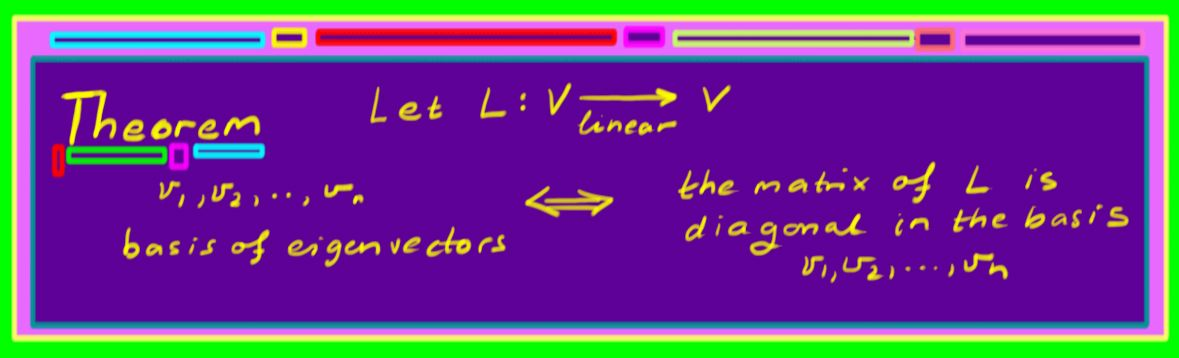
\includegraphics[scale=.33]{\diagPath/eigenbasis.jpg}
\end{center}
\caption{This theorem answers the question: ``What is diagonalization?''}
\end{figure}

%\section*{References}
%Hefferon, Chapter Three, Section V: Change of Basis
%\\
%Beezer, Chapter E, Section SD
%\\
%Beezer, Chapter R, Sections MR-CB
%\\
%Wikipedia:
%\begin{itemize}
%\item \href{http://en.wikipedia.org/wiki/Change_of_basis}{Change of Basis}
%\item \href{http://en.wikipedia.org/wiki/Diagonalizable_matrix}{Diagonalizable Matrix}
%\item \href{http://en.wikipedia.org/wiki/Similar_matrix}{Similar Matrix}
%\end{itemize}
%

\section{Review Problems}

{\bf Webwork:} 
\begin{tabular}{|c|c|}
\hline
Reading Problems & 
 \hwrref{Diagonalization}{1}, \hwrref{Diagonalization}{2}\\
No real eigenvalues &  \hwref{Diagonalization}{3}\\
Diagonalization &  \hwref{Diagonalization}{4}, \hwref{Diagonalization}{5},  \hwref{Diagonalization}{6},
 \hwref{Diagonalization}{7}\\
  \hline
\end{tabular}





\begin{enumerate}

\item Let $D=\begin{pmatrix}
\lambda_1 & \mc0 \\
\mc0 & \lambda_2 \\
\end{pmatrix}$.
\begin{enumerate}
\item Write $D$ in terms of the vectors $e_1$ and $e_2$, and their transposes.
\item Suppose $P=\begin{pmatrix}
a & b \\
c & d \\
\end{pmatrix}$ is invertible.  Show that $D$ is similar to
\[
M=\frac{1}{ad-bc}\begin{pmatrix}
\lambda_1ad-\lambda_2bc & -(\lambda_1-\lambda_2)ab \\[1mm]
(\lambda_1-\lambda_2)cd & -\lambda_1bc + \lambda_2ad
\end{pmatrix}.
\]
\item Suppose the vectors $\rowvec{a,b}$ and $\rowvec{c,d}$ are orthogonal.  What can you say about $M$ in this case? (Hint: think about what \(M^T\) is equal to.)
\end{enumerate}

\phantomnewpage

\item \label{orthogprob} Suppose $S=\{v_1, \ldots, v_n \}$ is an \emph{orthogonal} (not orthonormal) basis for~$\Re^n$.  Then we can write any vector $v$ as $v=\sum_ic^iv_i$ for some constants $c^i$.  Find a formula for the constants $c^i$ in terms of $v$ and the vectors in~$S$.

\Videoscriptlink{orthonormal_bases_hint.mp4}{Hint}{scripts_orthonormal_bases_hint}
\phantomnewpage

\item \label{orthogprojprob} Let $u,v$ be linearly independent vectors in $\Re^3$, and $P=\spa \{ u,v\}$ be the plane spanned by $u$ and $v$.  
\begin{enumerate}
\item Is the vector $v^\bot := v-\frac{u\cdot v}{u\cdot u}u$ in the plane $P$?
\item  What is the (cosine of the) angle between $v^\bot$ and $u$?
\item %Given your solution to the above, 
How can you find a third vector perpendicular to both $u$ and $v^\bot$?
\item  Construct an orthonormal basis for $\Re^3$ from $u$ and $v$.
\item  Test your abstract formul\ae\ starting with 
\[
u=\rowvec{1 , 2 , 0} \text{ and } v=\rowvec{0 , 1 , 1}.
\]
\end{enumerate}

\Videoscriptlink{orthonormal_bases_hint3.mp4}{Hint}{scripts_orthonormal_bases_hint3}

\phantomnewpage



\item Find an orthonormal  basis for $\Re^4$ which includes $(1,1,1,1)$ using the following procedure:\\
\begin{enumerate} 
\item Pick a vector perpendicular to the vector 
$$v_1 =\colvec{1\\1\\1\\1}$$ from the solution set of the matrix equation $$v_1^Tx=0\, .$$ Pick the vector $v_2$ obtained from the standard Gaussian elimination procedure which is the coefficient of $x_2$.
\item Pick a vector perpendicular to both $v_1$ and $v_2$ from the solutions set of the matrix equation $$\colvec{v_1^T\\[1mm]v_2^T}x=0\, .$$ Pick the vector $v_3$ obtained from the standard Gaussian elimination procedure with $x_3$ as the coefficient. 
\item Pick a vector perpendicular to $v_1,v_2,$ and $v_3$ from the solution set of the matrix equation $$\colvec{v_1^T\\[1mm]v_2^T\\[1mm]v_3^T}x=0\, .$$  Pick the vector $v_4$ obtained from the standard Gaussian elimination procedure with $x_3$ as the coefficient. 
\item Normalize the four vectors obtained   above.
\end{enumerate}


\item Use the inner product $$f\cdot g := \int_0^1 f(x)g(x)dx$$  on the vector space $V={\rm span} \{1,x,x^2,x^3\}$ to perform the Gram-Schmidt procedure on the set of vectors $\{1,x,x^2,x^3\}$. 

\item Use the inner product $$f\cdot g := \int_0^{2\pi} f(x)g(x)dx$$  on the vector space $V={\rm span} \{\sin(x),\sin(2x),\sin(3x) \}$ to perform the Gram-Schmidt procedure on the set of vectors $\{\sin(x),\sin(2x),\sin(3x) \}$. \\
Try to build an orthonormal basis for the vector space $$\spa \{ \sin(nx)~| ~n\in \N \}\, .$$
%What do you suspect about the vector space $\spa \{ \sin(nx)~| ~n\in \N \}$?\\
%What do you suspect about the vector space $\spa \{ \sin(ax)~|~ a \in \Re \}$?
\item 
\begin{enumerate}
\item
Show that if $Q$ is an orthogonal $n\times n$ matrix, then $$u\dotprod v = (Qu)\dotprod (Qv)\, ,$$ for any $u,v\in \Re^n$. That is, $Q$ preserves the inner product. 
\item Does $Q$ preserve the outer product? 
\item  If the set of vectors $\{ u_1,\dots,u_n\}$ is orthonormal and $\{ \lambda_1,\cdots,\lambda_n\}$ is a set of numbers, 
then what are the eigenvalues and eigenvectors of the matrix
$M=\sum_{i=1}^n \lambda_i u_i u_i^T$? 
\item How would the eigenvectors and eigenvalues of this matrix change if we replaced  $\{ u_1,\dots,u_n\}$ by $\{ Qu_1,\dots,Q u_n\}$?
\end{enumerate}


\item Carefully write out the Gram-Schmidt procedure for the set of vectors 
$$\left\{ \colvec{1\\1\\1}, \colvec{1\\-1\\1}, \colvec{1\\1\\-1} \right\} \, .$$ Is it possible to rescale the second vector obtained in the procedure to a vector with integer components? 


\item 
\label{basisortho}
\begin{enumerate}
\item Suppose $u$ and $v$ are linearly independent.  Show that $u$ and $v^\perp$ are also linearly independent.  Explain why $\{u, v^\perp\}$ is a basis for $\spa \{u,v\}$.



\Videoscriptlink{gram_schmidt_and_orthogonal_complements_hint.mp4}{Hint}{gram_schmidt_and_orthogonal_complements_hint}

\item Repeat the previous problem, but with three independent vectors $u,v,w$
 where $v^\perp$ and $w^\perp$ are as defined by the Gram-Schmidt procedure. 
\end{enumerate}

\phantomnewpage


\item \label{QRprob} Find the $QR$ factorization of
$$
M=\begin{pmatrix}1&0&\phantom{\!-}2\\-1&2&0\\-1&-2&2
\end{pmatrix}\, .
$$

\phantomnewpage

\item Given any three vectors $u,v,w$, when do $v^\perp$ or $w^\perp$ of the Gram--Schmidt procedure vanish?

\phantomnewpage

\item For $U$ a subspace of $W$, use the subspace theorem to check that $U^\perp$ is a subspace of $W$.

\phantomnewpage


\phantomnewpage

\item %(Extra Credit) 
Let $S_n$ and $A_n$ define the space of $n \times n$ symmetric and anti-symmetric matrices, respectively. These are subspaces of the vector space $M^n_n$ of all $n\times n$ matrices. What is $\dim M^n_n$, $\dim S_n$, and $\dim A_n$? Show that $M^n_n = S_n + A_n$. Define an inner product on square matrices
$$
M\cdot N ={\rm tr} MN\, .
$$
Is $A_n^{\perp}=S_n$? Is $M^n_n = S_n \oplus A_n$?

%\emph{Hint: Note that $\dim S_n = \dim U_n$ where $U_n$ is the vector space of all $n \times n$ upper triangular matrices, and also note that $\dim A_n = \dim \widetilde{U}_n$ where $\widetilde{U}_n$ is the vector space of all strictly $n \times n$ upper triangular matrices (\emph{i.e.} the diagonal entries are all 0).}

\item The vector space $V={\rm span} \{ \sin(t),\sin(2t), \sin(3t) , \sin(3t)\}$ has an inner product: 
$$f\cdot g:=\int _0^{2\pi}f(t)g(t) dt\, .$$ Find the orthogonal compliment to $U={\rm span} \{ \sin(t)+\sin(2t) \}$ in $V$. Express $\sin(t)-\sin(2t)$ as  the sum of vectors from $U$ and $U^\perp$.

\end{enumerate}

\phantomnewpage

\newpage

